\documentclass{article}

\usepackage[margin=1in]{geometry} 
\usepackage{amsmath,amsthm,amssymb}
\usepackage{graphicx}

\newcommand{\R}{\mathbb{R}}
\newcommand{\Z}{\mathbb{Z}}
\newcommand{\N}{\mathbb{N}}
\newcommand{\Q}{\mathbb{Q}}
\newcommand{\C}{\mathbb{C}}

\newenvironment{theorem}[2][Ejercicio]{\begin{trivlist}
\item[\hskip \labelsep {\bfseries #1}\hskip \labelsep {\bfseries #2.}]}{\end{trivlist}}
\newenvironment{lemma}[2][Lemma]{\begin{trivlist}
\item[\hskip \labelsep {\bfseries #1}\hskip \labelsep {\bfseries #2.}]}{\end{trivlist}}
\newenvironment{exercise}[2][Exercise]{\begin{trivlist}
\item[\hskip \labelsep {\bfseries #1}\hskip \labelsep {\bfseries #2.}]}{\end{trivlist}}
\newenvironment{problem}[2][Problem]{\begin{trivlist}
\item[\hskip \labelsep {\bfseries #1}\hskip \labelsep {\bfseries #2.}]}{\end{trivlist}}
\newenvironment{question}[2][Question]{\begin{trivlist}
\item[\hskip \labelsep {\bfseries #1}\hskip \labelsep {\bfseries #2.}]}{\end{trivlist}}
\newenvironment{corollary}[2][Corollary]{\begin{trivlist}
\item[\hskip \labelsep {\bfseries #1}\hskip \labelsep {\bfseries #2.}]}{\end{trivlist}}

\newenvironment{solution}{\begin{proof}[Solution]}{\end{proof}}

\begin{document}

\title{Métodos Numéricos de Optimización con restricciones.}
\author{Bustos Jordi\\Práctica II}

\maketitle

\begin{theorem}{1}
    Sean \(f : \mathbb{R}^n \to \mathbb{R}, x, d \in \mathbb{R}^n, \lambda > 0\) tales que
    \(x + \lambda d\) cumple la condición de Armijo. Sea \(0 < \mu < \lambda \).
    ¿Cumple \(\mu \) la condición de Armijo? Pruébelo o dé un contraejemplo que puede ser gráfico.
\end{theorem}

\begin{proof}
    Análogamente al ejemplo visto en clase podemos ver que no siempre se cumple la condición de Armijo para \( 0 < \mu < \lambda \) pues en este caso, si
    \( \mu \in (x_1, x_2) \) no se cumple la regla de armijo y sin embargo se vale que \( \mu < \lambda \). \\
    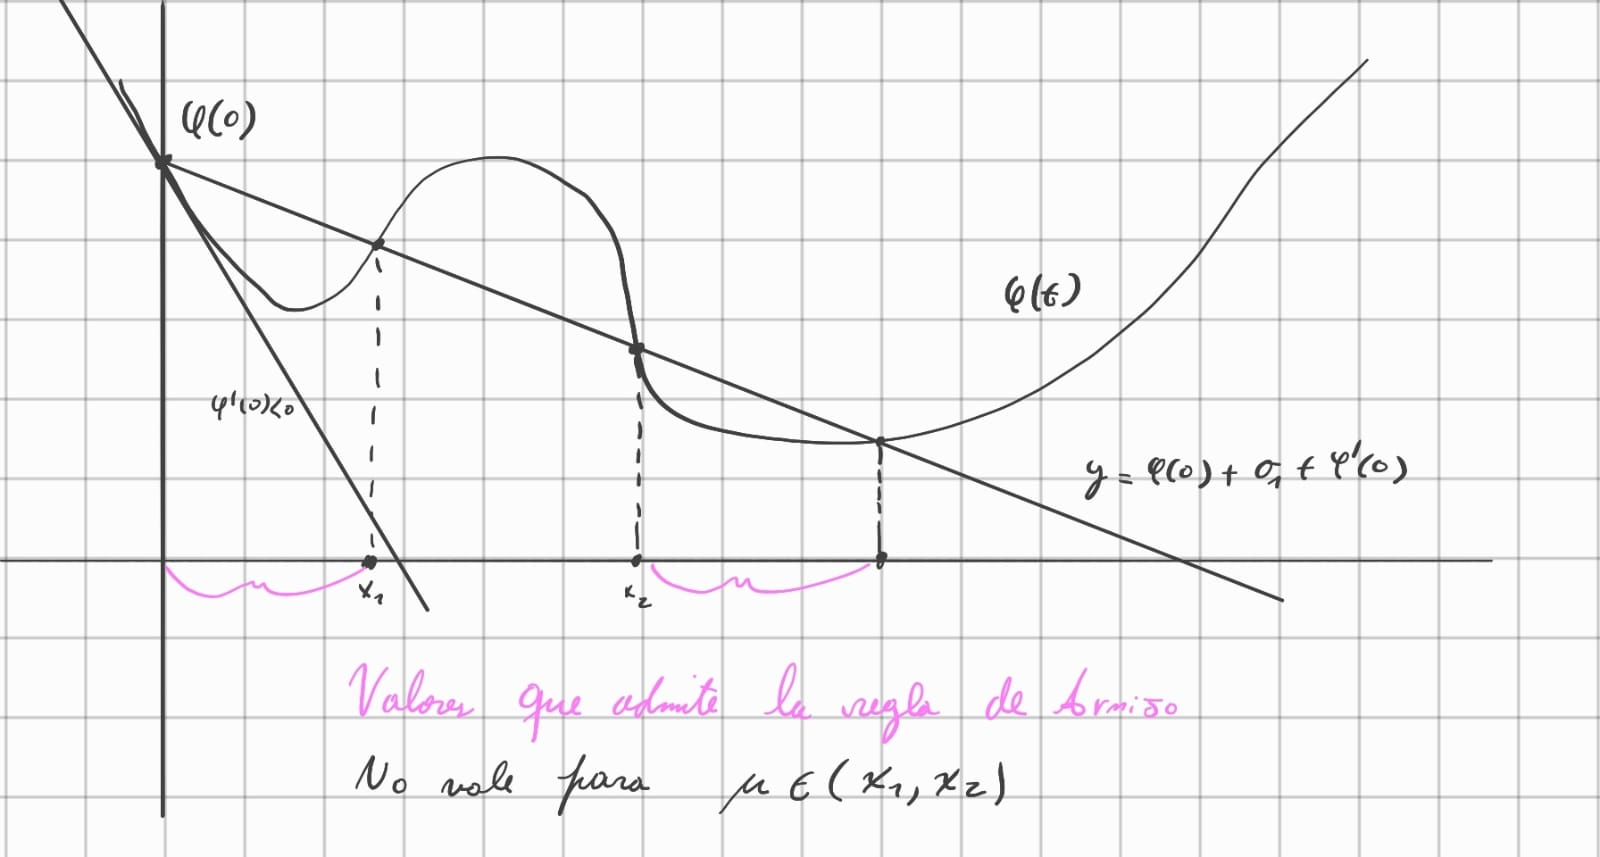
\includegraphics[width=14cm, height=8cm]{media/p2ej1.jpeg}
\end{proof}

\vspace{0.25in}

\begin{theorem}{2}
    Considere la función
    \[
        f(x,y) = x - y + 2x^2 + 2xy + y^2.
    \]

    \begin{itemize}
        \item[(a)] Muestre que \(d = (-1,0)\) es una dirección de descenso para \(f\) en \((0,0)\).
              Analizar cuál es el paso óptimo que se puede dar en esa dirección para hacer decrecer el
              valor de \(f\) utilizando búsqueda exacta.

        \item[(b)] Para la dirección de máximo decrecimiento en \((0,0)\) determinar el intervalo
              de paso máximo que se puede dar en esa dirección a partir de \((0,0)\) para hacer decrecer
              el valor de \(f\) utilizando la regla de Armijo con parámetro \(\sigma_1 = 1/4\).
    \end{itemize}
\end{theorem}

\begin{proof}
    Para demostrar (a) notemos que \( f \) es diferenciable y por lo tanto si \( {\nabla f(0,0)}^T \cdot d < 0 \implies d \) es una dirección de descenso. En efecto,
    sea \( d = (-1, 0) \): \begin{align*}
        \nabla{f(x,y)}            & = \begin{pmatrix}
                                          1 + 4x + 2y \\
                                          -1 + 2x + 2y
                                      \end{pmatrix} \\
        \nabla{f(0,0)}            & = \begin{pmatrix}
                                          1 \\
                                          -1
                                      \end{pmatrix} \\
        {\nabla f(0,0)}^T \cdot d & = -1 < 0
    \end{align*}
    Para hallar la longitud del paso óptimo, definimos \( \phi(t) = f((0,0) + t \cdot d) = f(-t, 0) = -t + 2t^2 \), luego \( \phi'(t) = -1 + 4t = 0 \iff t = \frac{1}{4} \) que es la longitud de paso óptima en la dirección \( d \). \\
    Para la parte (b) consideremos la regla de Armijo: \begin{align*}
        f(x + t d) & \leq f(x) + \sigma_1 t {\nabla f(x)}^T d
    \end{align*}
    La dirección de máximo decrecimiento está dada por \( - \nabla f(0,0) = (-1, 1) \), si \( \sigma_1 = \frac{1}{4} \) la regla de Armijo se traduce en: \begin{align*}
        f((0,0) + t \cdot (-1, 1)) & \leq f(0, 0) + \frac{1}{4} t {\nabla f(0,0)}^T \cdot (-1, 1) \\
        f(-t, t)                   & \leq \frac{1}{4} t \cdot (-2)                                \\
        t^2 - 2t                   & \leq -\frac{1}{2} t                                          \\
        t^2 - \frac{3}{2} t        & \leq 0                                                       \\
        t(t - \frac{3}{2})         & \leq 0
    \end{align*}
    Por lo tanto, el intervalo de paso máximo es \( (0, \frac{3}{2}] \).
\end{proof}

\vspace{0.25in}

\begin{theorem}{3}
    Considere la función
    \[
        f(x,y) = 2x^2 + y^2 - 2xy + 2x^3 + x^4.
    \]

    \begin{itemize}
        \item[(a)] Verificar que \(d = (0,1)\) es una dirección de descenso para \(f\) a partir de \((0,-2)\).

        \item[(b)] Para la dirección a partir de \((0,-2)\) considerada en (a), el valor \(t=1\) verifica
              la regla de Armijo con parámetro \(\sigma_1 = 4/5\)?
              ¿Para qué valores de \(\sigma_1\) el valor de longitud de paso \(t=1\) verifica la regla de Armijo?
    \end{itemize}
\end{theorem}

\begin{proof}
    Análogamente al ejercicio anterior, para (a) se tiene que, dado \( d = (0, 1) \): \begin{align*}
        \nabla f(x,y)              & = \begin{pmatrix}
                                           4x - 2y + 6x^2 + 4x^3 \\
                                           2y - 2x
                                       \end{pmatrix} \\
        \nabla f(0,-2)             & = \begin{pmatrix}
                                           4 \\
                                           -4
                                       \end{pmatrix}        \\
        {\nabla f(0,-2)}^T \cdot d & = -4 < 0
    \end{align*}
    Luego, \( d \) es una dirección de descenso para \( f \) en \( (0, -2) \). \\
    Para (b) consideremos la regla de Armijo con \( \sigma_ 1 = \frac{4}{5} \) y \( t = 1 \): \begin{align*}
        f((0,-2) + 1 \cdot (0,1)) & \leq f(0, -2) + \frac{4}{5} \cdot 1 \cdot {\nabla f(0,-2)}^T \cdot (0,1) \\
        f(0, -1)                  & \leq f(0, -2) + \frac{4}{5} \cdot (-4)                                   \\
        1                         & \leq 4 - \frac{16}{5}                                                    \\
        1                         & \leq \frac{4}{5}
    \end{align*}
    Absurdo, luego \( t = 1 \) no verifica la regla de Armijo con \( \sigma_1 = \frac{4}{5} \). \\
    Para hallar los valores de \( \sigma_1 \) para los cuales \( t = 1 \) verifica la regla de Armijo, consideremos: \begin{align*}
        1        & \leq 4 + \sigma_1 \cdot (-4) \\
        \sigma_1 & \leq \frac{3}{4}
    \end{align*}
    Por lo tanto, \( t = 1 \) verifica la regla de Armijo para \( \sigma_1 \in (0, \frac{3}{4}] \).
\end{proof}

\vspace{0.25in}

\begin{theorem}{4}
    Sea \(f\) una función diferenciable tal que \(\nabla f(x) \neq 0\).
    Mostrar que si \(H : \mathbb{R}^n \to \mathbb{R}^{n \times n}\) es una función continua que asigna a
    cada \(x \in \mathbb{R}^n\) una matriz definida positiva \(H(x)\) entonces la dirección
    \[
        d = - H(x) \nabla f(x)
    \]
    es una dirección de descenso para \(f\) en \(x\).
\end{theorem}

\begin{proof}
    Como la matriz  \( H(x) \) es definida positiva y \( \nabla f(x) \neq 0 \) se tiene que \begin{align*}
        {\nabla f(x)}^T \cdot H(x) \cdot \nabla f(x)  & > 0 \\
        -{\nabla f(x)}^T \cdot H(x) \cdot \nabla f(x) & < 0 \\
        {\nabla f(x)}^T \cdot d                       & < 0
    \end{align*}
    y como \( f \) es diferenciable \( d = - H(x) \nabla{f(x)} \) es una dirección de descenso.
\end{proof}

\vspace{0.25in}

\begin{theorem}{5}
    Considere la función \( f(x,y) = {(x - 2y)}^2 + x^4 \).
    Calcular la dirección de Newton en el punto \((2,1)\).
    ¿Cumple el valor \(t = 1\) la regla de Armijo con parámetro \(\sigma_1 = 1/5\)?
\end{theorem}

\begin{proof}
    Por definición de dirección de Newton buscamos: \begin{align*}
        \nabla^2 f(2, 1) \cdot d & = - \nabla f(2, 1) \\
    \end{align*}
    Donde \begin{align*}
        \nabla f(x,y)   & = \begin{pmatrix}
                                2(x - 2y) + 4x^3 \\
                                -4(x - 2y)
                            \end{pmatrix} \\
        \nabla f(2,1)   & = \begin{pmatrix}
                                16 \\
                                0
                            \end{pmatrix}   \\
        \nabla^2 f(x,y) & = \begin{pmatrix}
                                2 + 12x^2 & -4 \\
                                -4        & 8
                            \end{pmatrix}   \\
        \nabla^2 f(2,1) & = \begin{pmatrix}
                                50 & -4 \\
                                -4 & 8
                            \end{pmatrix}
    \end{align*}
    Por lo tanto, \begin{align*}
        \begin{pmatrix}
            50 & -4 \\
            -4 & 8
        \end{pmatrix} \cdot d & = \begin{pmatrix}
                                      -16 \\
                                      0
                                  \end{pmatrix} \\
        d                     & = \begin{pmatrix}
                                      -\frac{1}{3} \\
                                      -\frac{1}{6}
                                  \end{pmatrix}
    \end{align*}
    Una vez más, recordemos la regla de Armijo: \begin{align*}
        f(x + t \cdot d) & \leq f(x) + \sigma_1 t {\nabla f(x)}^T \cdot d
    \end{align*}
    En particular,\begin{align*}
        f((2,1) + 1 \cdot (-1/3, -1/6)) & \leq f(2, 1) + \frac{1}{5} \cdot 1 \cdot {\nabla f(2,1)}^T \cdot (-1/3, -1/6) \\
        {\left (\frac{5}{3} \right)}^4  & \leq 16 - \frac{16}{15}                                                       \\
    \end{align*}
    Que es verdadero, luego \( t = 1 \) cumple la regla de Armijo con \( \sigma_1 = \frac{1}{5} \).
\end{proof}
\vspace{0.25in}

\begin{theorem}{6}
    Considere el siguiente método:
    \begin{itemize}
        \item Dado \(x_k\). Calcular \(d_k\) como se indica a continuación.
        \item Hacer \(t = 1\).

              Si \( f(x_k + t d_k) \leq f(x_k) + \tfrac{1}{2} t d_k^T \nabla f(x_k) \) \((*)\) hacer
              \( x_{k+1} = x_k + t d_k \),

              Sino, reemplazar por \(t/2\) hasta que se verifique \((*)\).
    \end{itemize}

    Sea \( f(x,y) = x^2 + y^2 - xy, \; x_0 = (2,0) \).
    \begin{enumerate}
        \item[(a)] Dibuje algunas curvas de nivel de \(f\).
        \item[(b)] Hacer dos iteraciones del método utilizando la dirección de Cauchy. Dibuje los iterados obtenidos en el plano en el cual están las curvas de nivel de \(f\).
        \item[(c)] Resuelva el problema mediante el uso de la dirección de Newton.
    \end{enumerate}
\end{theorem}

\begin{proof}

\end{proof}
\vspace{0.25in}

\begin{theorem}{7}
    Sean \(u, v \in \mathbb{R}^n\) no nulos y \(A \in \mathbb{R}^{n \times n}\) una matriz no singular.
    Sea \( B = A + u v^T \). Demuestre que \(B\) es no singular si y solo si
    \(\sigma = 1 + v^T A^{-1} u \neq 0\). En este caso demuestre que
    \[
        B^{-1} = A^{-1} - \tfrac{1}{\sigma} A^{-1} u v^T A^{-1}.
    \]

    \textbf{Idea de la demostración:}
    \begin{enumerate}
        \item[(a)] Mostrar que la matriz \(B = I + xy^T\), para \(x,y \in \mathbb{R}^n\)
              tiene dos autovalores: \(\lambda_1 = 1\) con multiplicidad \(n-1\)
              (hay que demostrar que \(\dim(\text{Nú}(B - \lambda_1 I)) = n-1\),
              para eso considerar que la imagen de \(B - \lambda_1 I = xy^T\) que es una matriz de rango 1
              cuya imagen tiene dimensión 1) y \(\lambda_2 = 1 + y^T x\).

        \item[(b)] Lo anterior implica que
              \[
                  \det(B) = 1 + y^T x,
              \]
              luego,
              \[
                  \det(I + A^{-1} x y^T) = 1 + y^T A^{-1} x.
              \]

        \item[(c)] Finalmente mostrar que \(A + uv^T\) es no singular si y solo si
              \(I + A^{-1} u v^T = A^{-1} (A + uv^T)\) es invertible.
              Luego, hacer el producto de la matriz por su inversa para verificar la fórmula.
    \end{enumerate}
\end{theorem}

\begin{proof}

\end{proof}
\vspace{0.25in}

\begin{theorem}{8}
    Demostrar que la adaptada BFGS para la inversa cumple:
    Si \(H_k\) es simétrica definida positiva y se tiene que \(s_k^T y_k > 0\)
    entonces \(H_{k+1}\) es simétrica definida positiva.
\end{theorem}

\begin{proof}

\end{proof}
\vspace{0.25in}

\begin{theorem}{9}
    Considere el método de Quasi-Newton con fórmula adaptada secante DFP de rango 2
    con búsqueda lineal exacta y matriz inicial \(H_0\) definida positiva.
    Demuestre que \(y_k^T s_k > 0\) para todo \(k\).
    Ídem si se utiliza la búsqueda de Wolfe.
\end{theorem}

\begin{proof}

\end{proof}
\vspace{0.25in}

\end{document}